
%%%%%%%%%%%%%%%%%%%%%%%%%%%%%%%%%%%%%%%%%%%%%%
\section{Photon Detection System (PDS)}
\label{sec:pd_system}

LAr is an excellent scintillating medium and the photon detection
system will exploit this property in the detector.  With an
average energy of 19.5~eV needed to produce a photon (at zero field),
a typical particle depositing 1~MeV in LAr will generate
40,000~photons with wavelength of 128~nm. At higher fields this will
be reduced, but at 500~V/cm the yield is still $\sim$20,000~photons
per MeV. Roughly 1/4 of the photons are promptly emitted with a
lifetime of about 6~ns while the rest have a lifetime of
1100--1600~ns. Prompt and delayed photons are detected in
  precisely the same way by the photon detection system. LAr is
highly transparent to the 128-nm VUV photons with a Rayleigh
scattering length of (66~$\pm$~3)~cm~\cite{Rayleigh} and absorption
length of $>$200~cm; this attenuation length requires a LN$_2$
  content of less than 20~ppm. The relatively large light output makes
the scintillation process an excellent candidate for determining the
$t_0$ for non-beam related events. Detection of the scintillation
light may also be helpful in background rejection and triggering on
non-beam events.

%%%%%%%%%%%%%%%%%%%%%%%%
\subsection{Scope and requirements}

The photon detector system (PDS) 
includes the following components:

\begin{itemize}
\item Light collection system including wavelength shifter and light guides
\item Light sensors: Silicon photo-multipliers (SiPMs)
\item Readout electronics
\item Monitoring system
\item Related infrastructure (frames, mounting boards, etc.).
\end{itemize}


The primary requirement is the detection of light from proton decay
candidates (as well as beam neutrino events) with high efficiency to
enable 3D spatial localization of candidate events. The light yield that
has been required for this is 0.1\,pe/MeV at the cathode plane.
The TPC will provide supernova neutrino detection, while the detection of light
from supernova neutrino interactions should localize the events and disentangle
them from background noise in the TPC detection.
The photon system will provide the $t_0$ timing of
events relative to TPC timing with a resolution better than 1~$\mu$s
(providing position resolution along the drift direction of a couple of mm). 
Measurements %from the ProtoDUNE-SP detector 
will determine the absolute
light yield by measuring light from beam particles and cosmic ray muons
tracked in the TPC or identified by external muon trigger counters.
Informed by this light yield measurement the determination of whether the 
light yield is sufficient for the required science goals can be made.

Figure~\ref{fig:PD_overview} shows the layout for the photon detector
system described in this section. %, which will be described in the following sections.

\begin{cdrfigure}[Photon detection system overview]{PD_overview}{Overview of the PDS
    system showing a cartoon schematic (a) of a single PDS module
    in the LAr and the channel ganging scheme used to reduce the
    number of readout channels. Panel (b) shows how each PDS module
    will be inserted into an APA frame. There will be 10 photon detectors (PDs) inserted
    into an APA frame.}
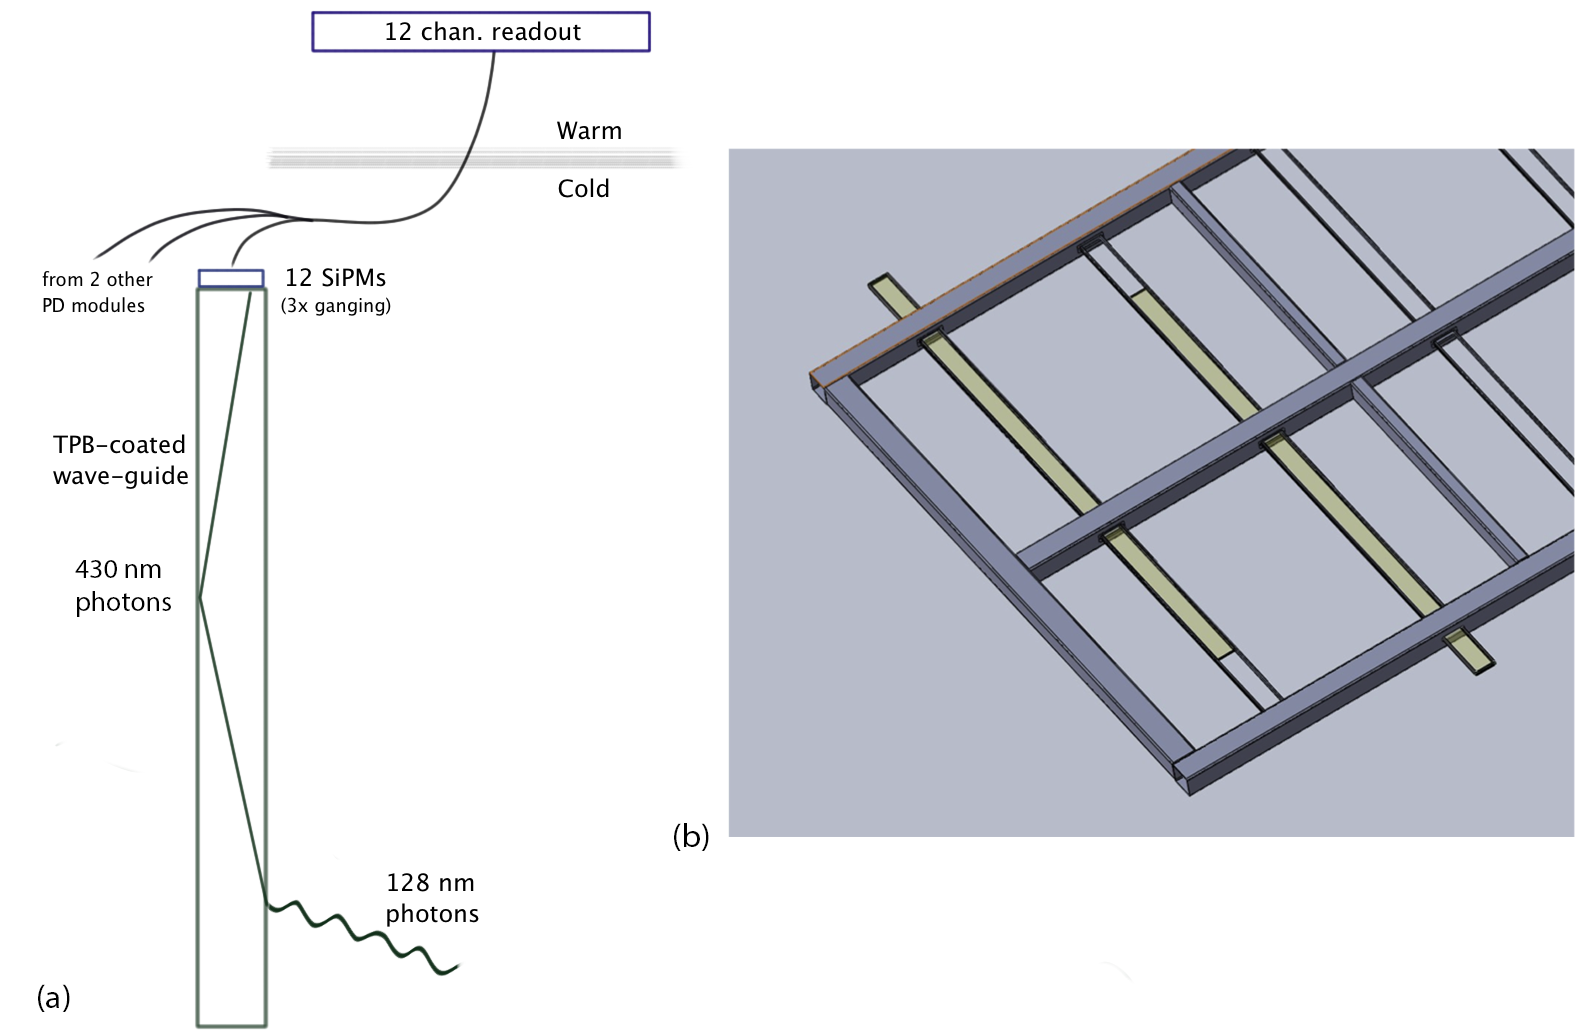
\includegraphics[width=1.0\linewidth]{pd_schem.png}
\end{cdrfigure}

%%%%%%%%%%%%%%%%%%%%%%%%%%
\subsection{Photon detector modules}

Two styles of PDS %photon detector (PD) 
modules are being produced for ProtoDUNE-SP.  
The concepts are very similar, but differ in the number of times the LAr scintillation 
light is shifted.  

The reference design shown schematically in Figure~\ref{fig:PD_overview}
has wavelength-shifting radiator plates mounted on a wavelength-shifting light guide.
The plates are coated 
with tetraphenyl-butadiene (TPB) to produce blue ($430nm$) light from the $128nm$ VUV 
scintillation light.  
This blue light is absorbed by a commercially produced wavelength shifting (WLS)
polystyrene bar with Y-11 fluor.  
The bar serves as a light guide to transmit the green light to the photosensor 
mounted at its end.
The radiator plates are captive in mounting blocks that are glued to the WLS bar
at regular intervals as shown in Figure~\ref{fig:PD_radiator_mount}.

\begin{cdrfigure}[Radiator Plate Mounting Blocks]{PD_radiator_mount}
  {Mounting of the radiator plates to the WLS bar for the reference design scheme}
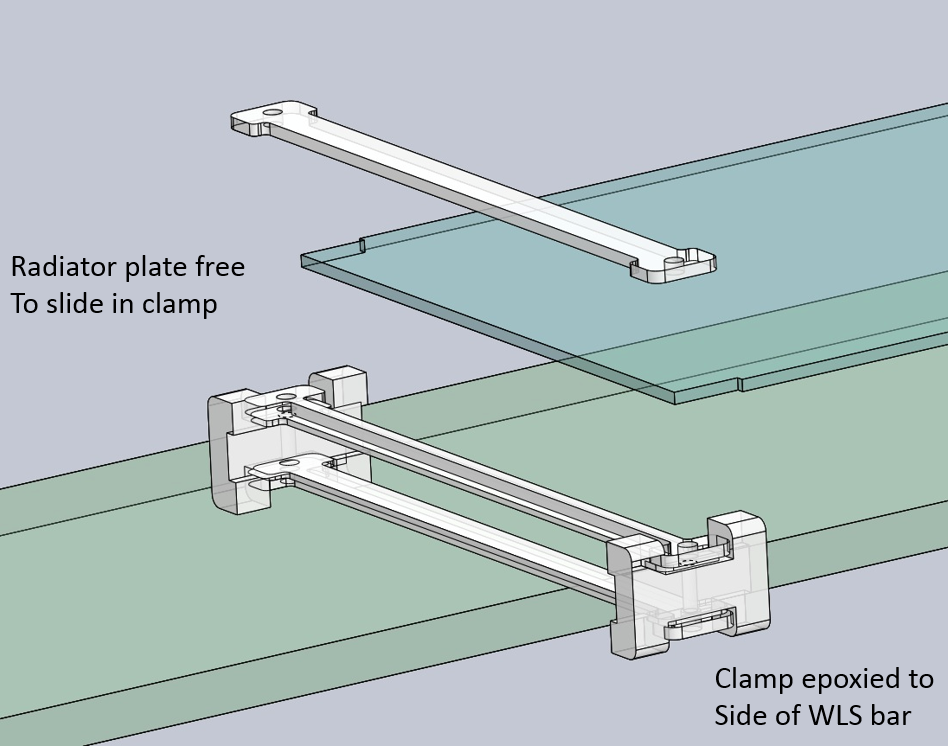
\includegraphics[width=0.5\linewidth]{PD_radiator_mount.PNG}
\end{cdrfigure}

The alternative design uses the same photodetector and mounting, but does not have
any radiator plates mounted on it.  
Instead, the bar is made by dip-coating an acrylic light guide with a solution
of TPB, solvents, and a surfactant to produce a bar with the wavelength shifter coated
on the outside.  
It has only one wavelength shifting step, which should increase the efficiency.  
Previous work for DUNE with this technique showed that the attenuation length, and
therefore the light yield, would suffer from the coating process, but bars produced with
the latest technique as shown in~\cite{conrad_jinst2015} have %been shown to have 
avoided this problem.




%%%%%%%%%%%%%%%%%%%%%%%%%%
\subsection{Sensors}
The planned photodetector is a SiPM, model 
%The model planned for ProtoDUNE-SP is the 
SensL C-Series 6~mm$^2$
(MicroFB-60035-SMT). % device. 
This model of SiPM has a detection efficiency of
41\%; the detection efficiency combines QE and effective area
  coverage accounting for dead space between pixels.   At LAr temperature (89~K) the dark rate is of order 10~Hz
(0.5 p.e. threshold) while after-pulsing has not been an
issue. Extensive testing is underway and will continue, to ensure 
that the SiPMs can reliably survive the stresses associated with 
any thermal cycling in LAr and long-term operation at LAr temperature.

All photodetectors %for ProtoDUNE-SP 
will be subjected to testing to determine
 forward and reverse bias I-V curves,
 breakdown voltage, dark current and dark count rate, photodetector gain, crosstalk estimation, response, and bias dependence of parameters.
 
%All SiPMs 
Each SiPM will be tested before mounting on the readout boards to determine
if the part meets the specifications in a warm test.  After mounting to
the readout board all items will be tested both warm and cold (cyrogenic 
temperature) to determine the operating characteristics as when %they will be 
installed in the %at the ProtoDUNE-SP 
detector, and during QA/QC tests on the PDS modules.

In addition to these tests, the photodetectors will be tested for their
response to light signals from an LED with appropriate wavelength.
These tests will be sensitive enough to determine if one of the three SiPM
elements in parallel is not functioning.


%%%%%%%%%%%%%%%%%%%%%%%%%%
\subsection{Mechanical design and installation}
  % -- CSU  -- Dave
  %  Mechanical Design Mounting 

The PDS system is configured as a set of \textit{modules} that are mounted on the APA frames.  A PDS module is
the combination of one light guide (also called a ``bar'' due to its
shape) and 12 SiPMs, as shown in Figure~\ref{fig:PD_overview}~(a). 
 %To enable this, the the reference design for mounting the PDs onto the
The reference design for the APA frames calls for ten PDS modules per APA, approximately 2.2-m long,
86-mm wide and 6-mm thick, equally spaced along the full length of the
APA frame, as shown in Figure~\ref{fig:PD_overview}~(b). 
The light guides are inserted into the APA frame on rails gliding on their radiator
plate mounting blocks, as shown in Figure~\ref{fig:PD_mounting_inslide} (right). \fixme{check if right figure ref}

\begin{cdrfigure}[Diagram of PDS installation into APA frame and installed SiPM mounting board]
  {PD_mounting_inslide}{(left) Rendering of the installation of a PDS module
    into an APA frame, shown just before it comes to rest on the inside face
    of the APA tube. (right) Rendering of the the SiPM mounting board
    installed on the end of the PDS module before insertion.}
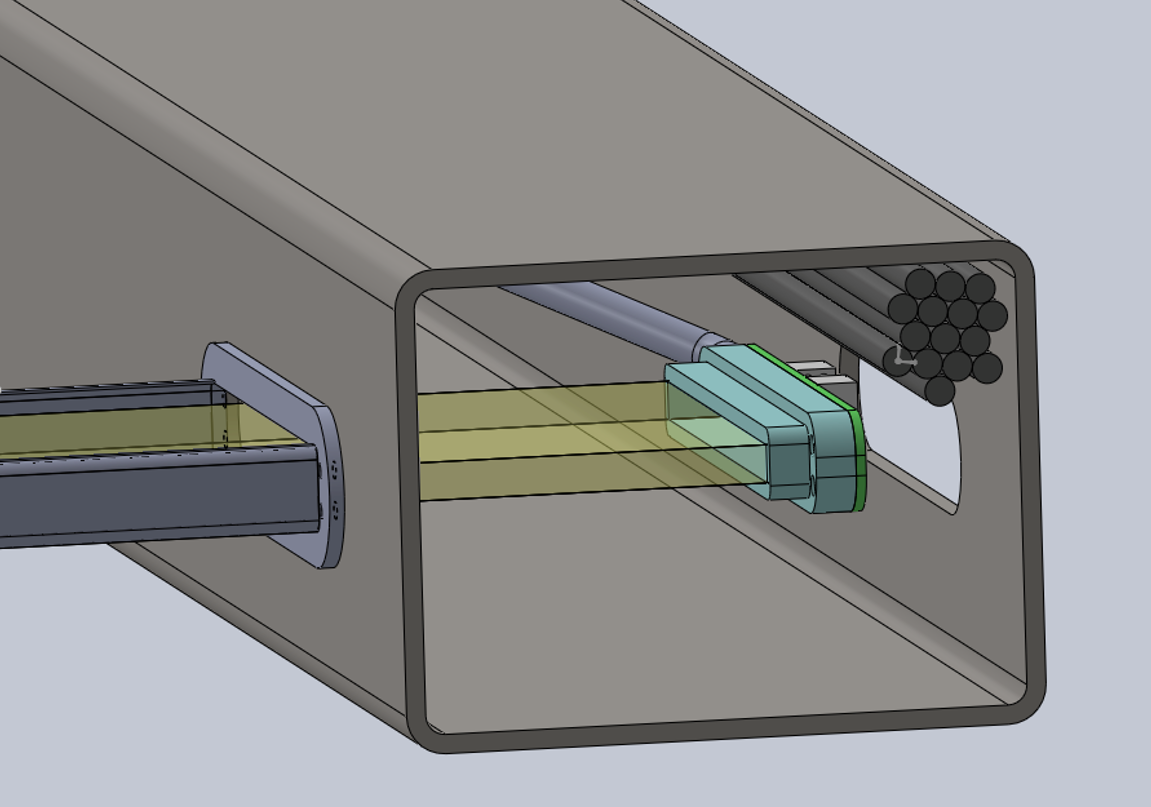
\includegraphics[width=0.456\linewidth]{PD_mounting_inslide.PNG}
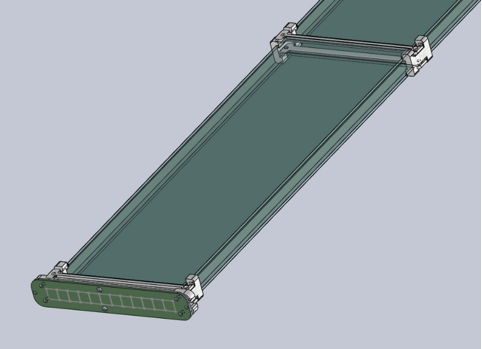
\includegraphics[width=0.444\linewidth]{PD_endblock_mnt.PNG}
\end{cdrfigure}
%
%\begin{cdrfigure}[SiPM mounting board attached to PDS module]
 % {PD_endblock_mnt.PNG}{Rendering of the the SiPM mounting board
  %  installed on the end of the PDS module before insertion.}
%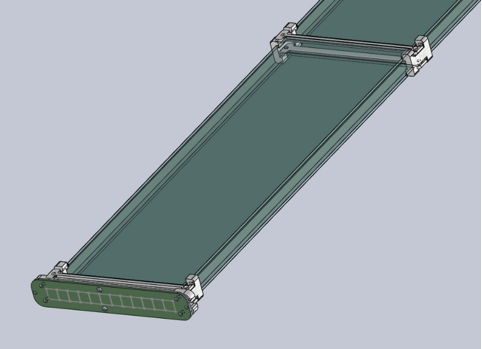
\includegraphics[width=0.50\linewidth]{PD_endblock_mnt.PNG}
%\end{cdrfigure}


The system has been prototyped and test fitted with a module at CSU 
as shown in Figure~\ref{fig:PD_flat_installtest}.
\begin{cdrfigure}[Photo of PD mock installation]
  {PD_flat_installtest}{Photograph of the installation
    test of a mock PDS module in a 1/5 section of an APA frame.}
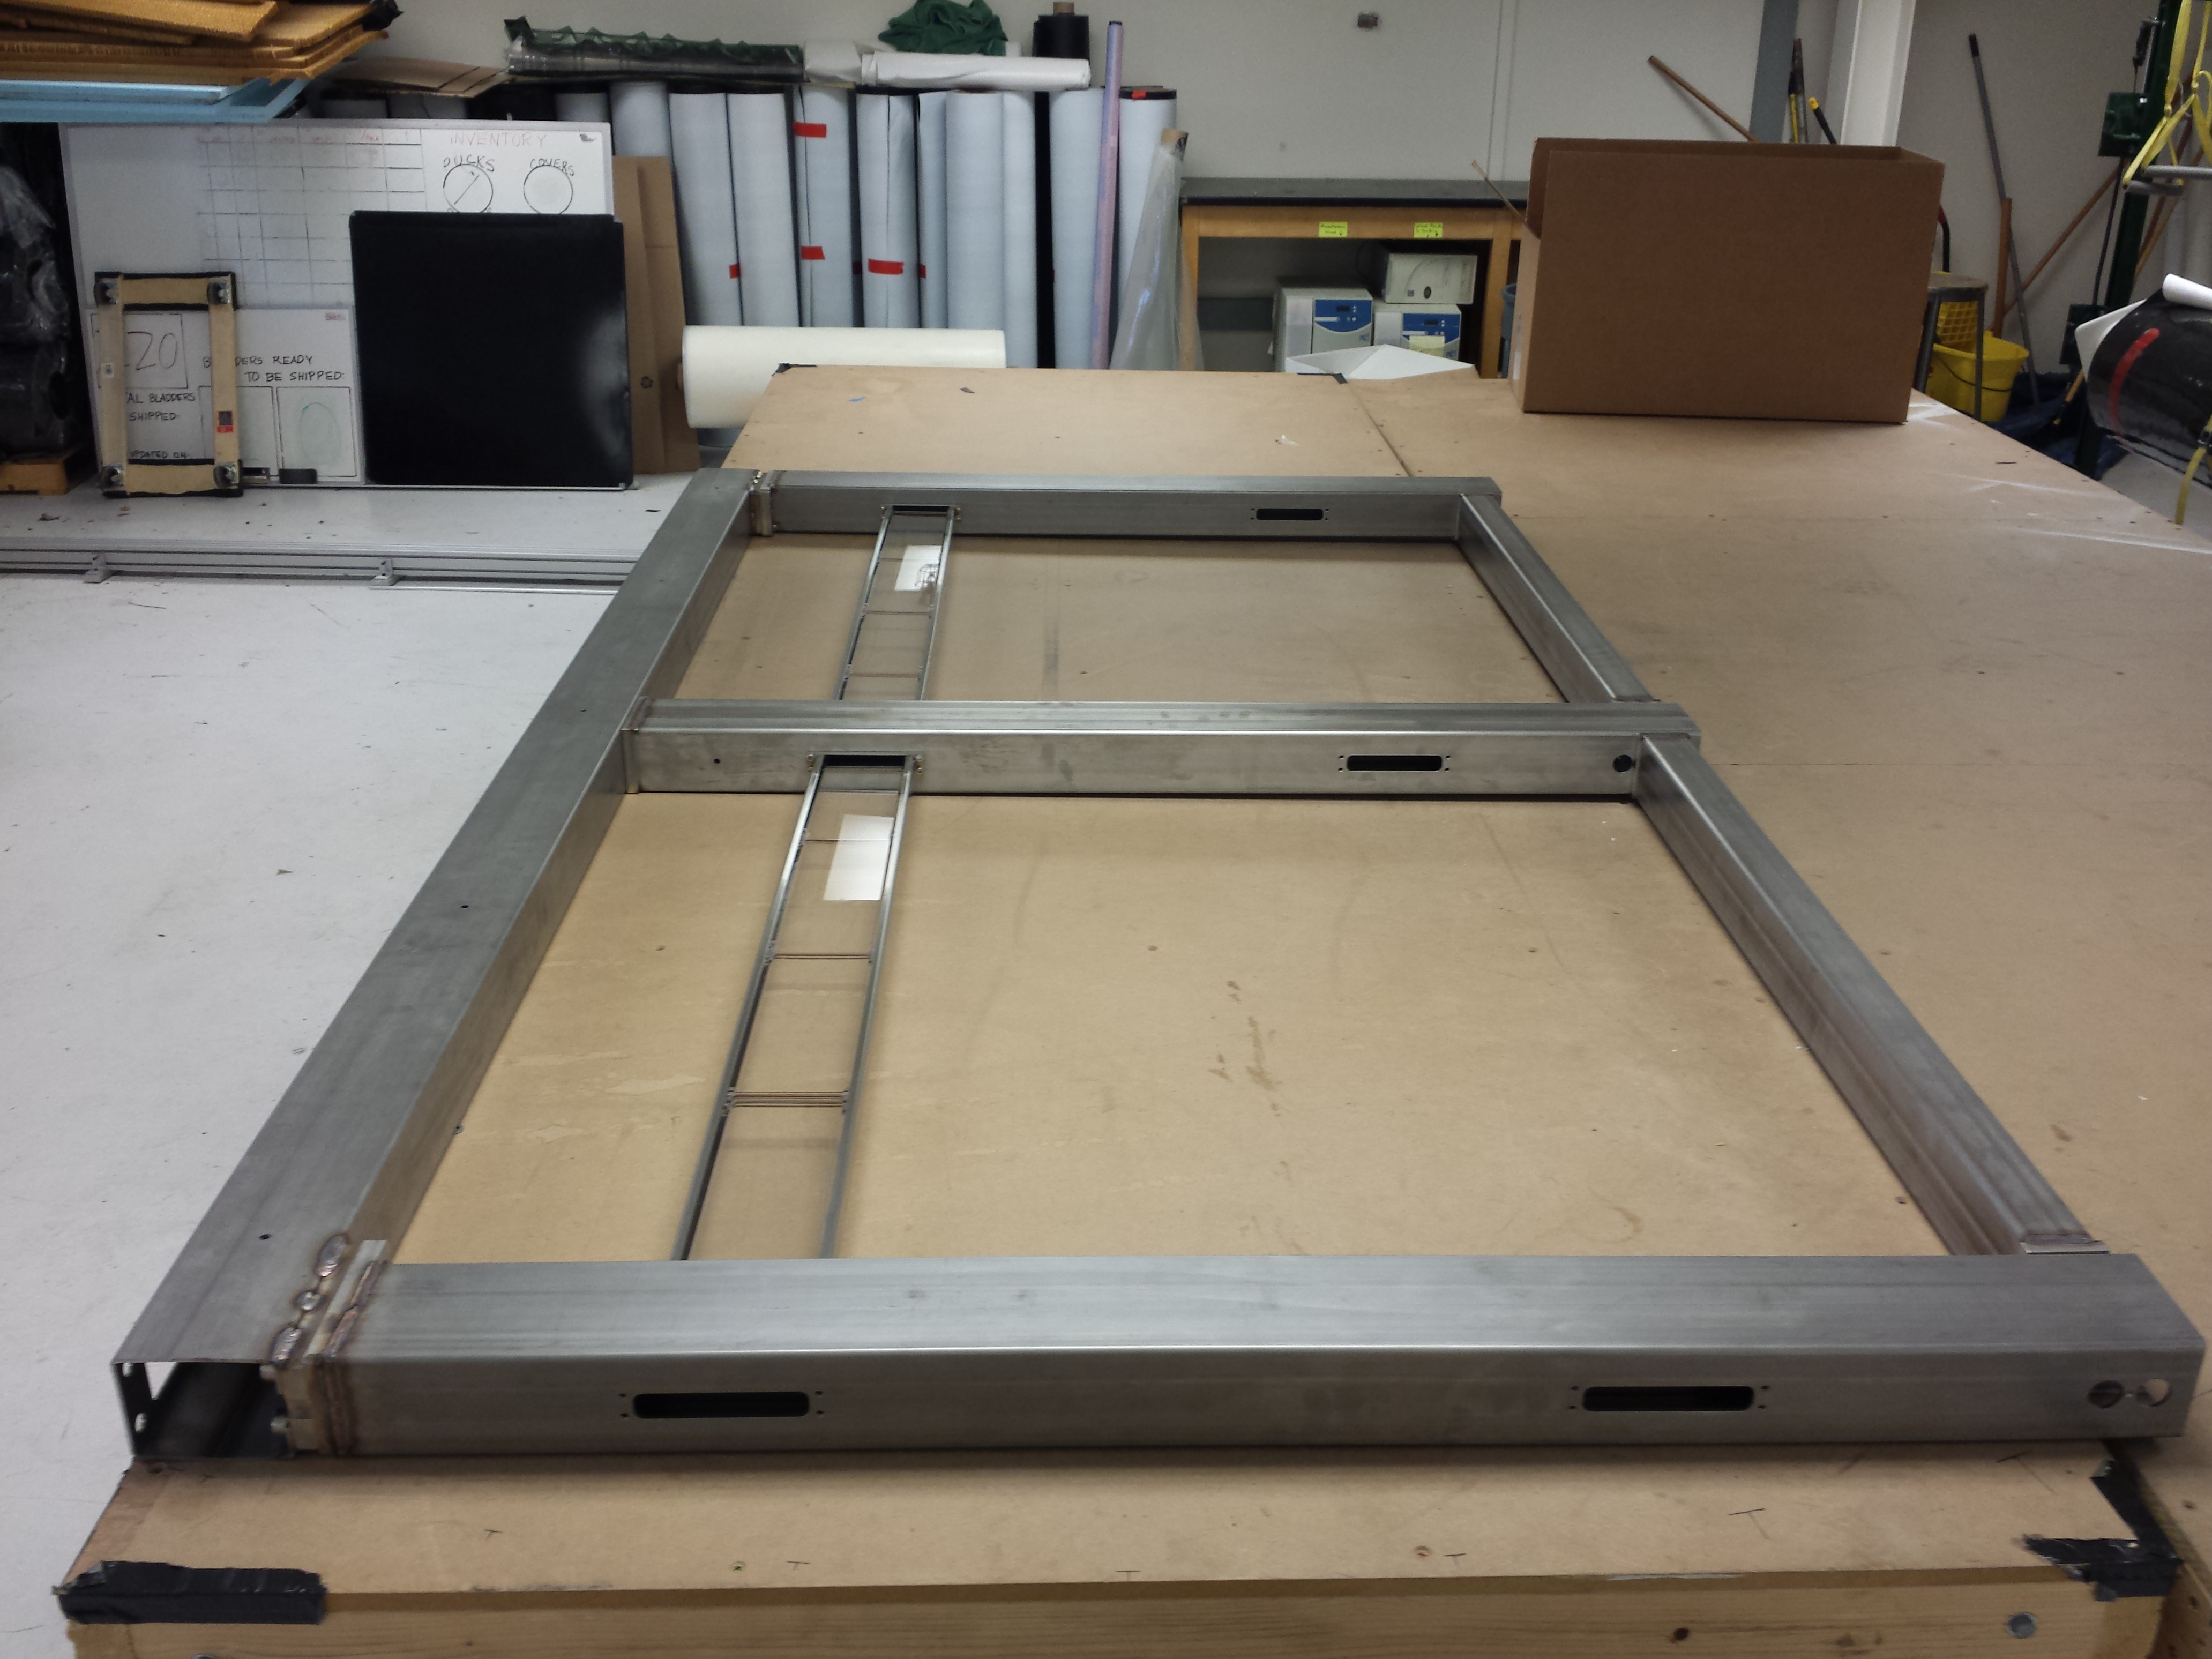
\includegraphics[width=0.50\linewidth]{pd_flat_installtest.jpg}
\end{cdrfigure}

  %   Mechanical Design SiPM mounting board

Each photon detector has a single SiPM mounting board with 12 surface-mount SiPMs 
mounted on the face as in Figure~\ref{fig:PD_SiPM_PCB_front} (left).
Four groups of $3$ SiPM elements will go to a single 
channel of readout electronics in order to reduce the cost of the readout.
The board is held close to the bar, without touching, by four screws that go into 
tapped holes on the end mounting block that is glued to the bar.  
The mounting block assembly is shown in Figure~\ref{fig:PD_mounting_inslide} (right) %\ref{fig:PD_endblock_mnt}.
The circuit board also has holes at each end for mounting to the APA frame.  

\begin{cdrfigure}[SiPM mounting board with 12 SiPMs and with Rj-45 connector]
  {PD_SiPM_PCB_front}{Photograph of a SiPM mounting board
    with the full complement of 12 SiPMs installed on the board (left), and with the 
    RJ-45 connector for the cable (right).}
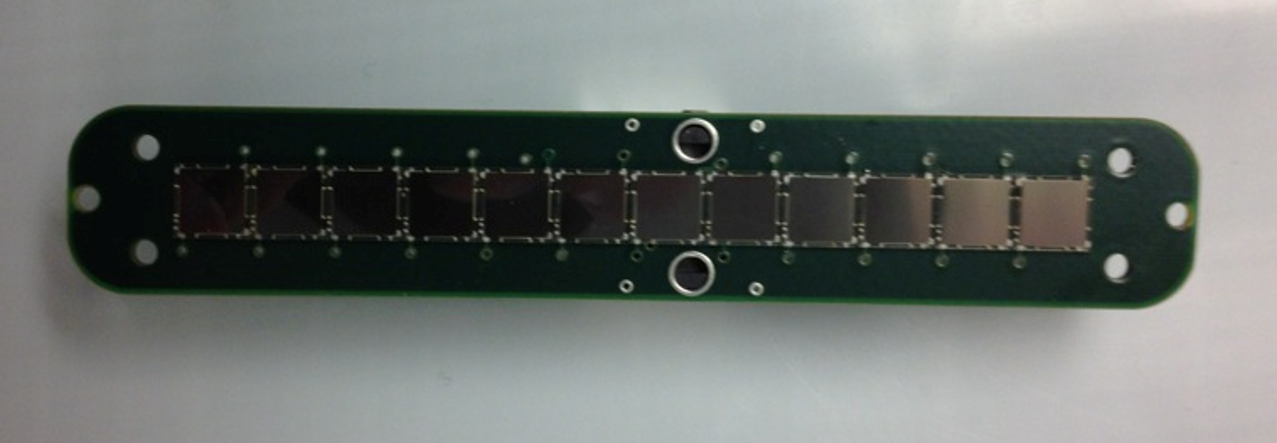
\includegraphics[width=0.55\linewidth]{PD_SiPMMountPCB_front.PNG}
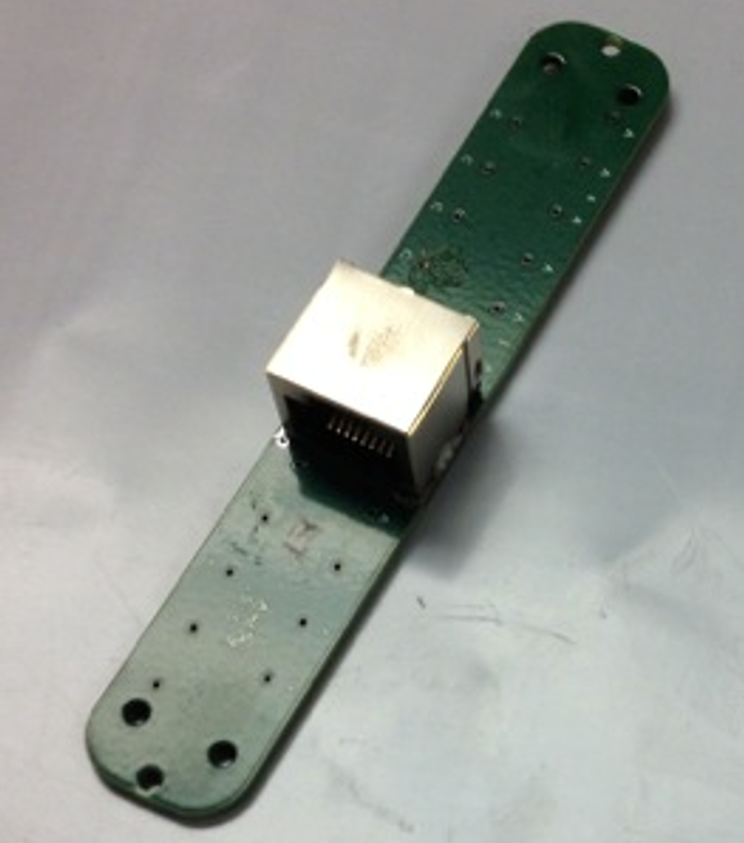
\includegraphics[width=0.4\linewidth]{PD_SiPMMountPCB_back.PNG}
\end{cdrfigure}
%\begin{cdrfigure}[Readout board with RJ-45 connector]
%  {PD_SiPMMountPCB_back}{Photograph of the SiPM readout PCB with the 
%    RJ-45 connector for the cable.}
%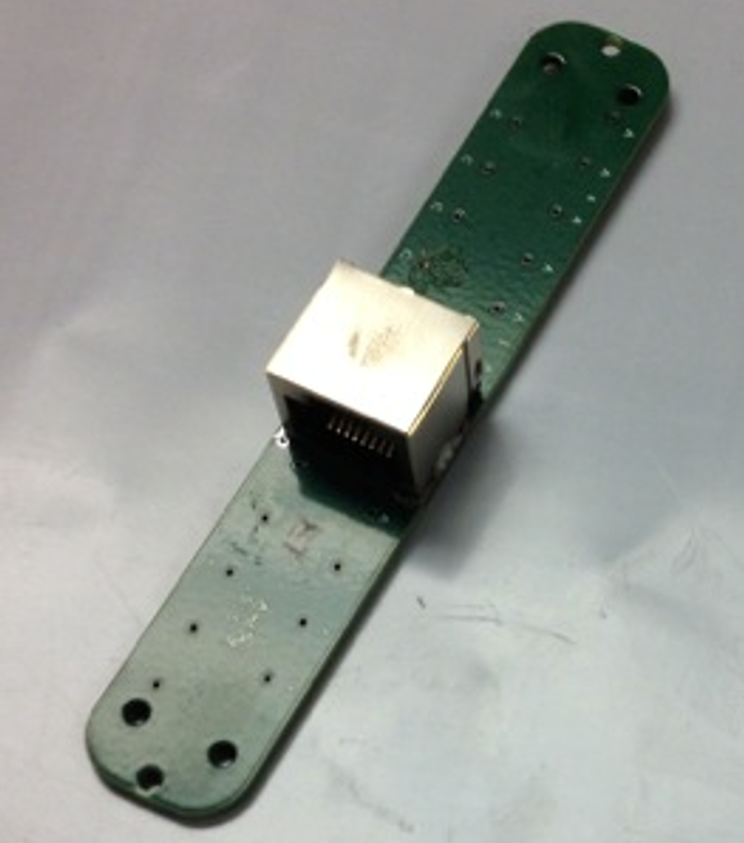
\includegraphics[width=0.50\linewidth]{PD_SiPMMountPCB_back.PNG}
%\end{cdrfigure}

  %   Mechanical Design Cabling

The cabling plan for the system has one cable with four shielded twisted pairs 
connected to each SiPM mounting board via the surface mount RJ-45 connector
shown mounted on the back of the readout PCB in 
Figure~\ref{fig:PD_SiPM_PCB_front} (right).  
The cables run through the APA tubing to the top of the APA frame as seen
in Figure~\ref{fig:PD_cable_intube}.
The cable bundles are installed and connected to each PD 
after the PD has been installed into the slot.
\begin{cdrfigure}[Cables in APA frame]
  {PD_cable_intube}{Diagram showing the routing of the PDS cables
    through the APA frame.}
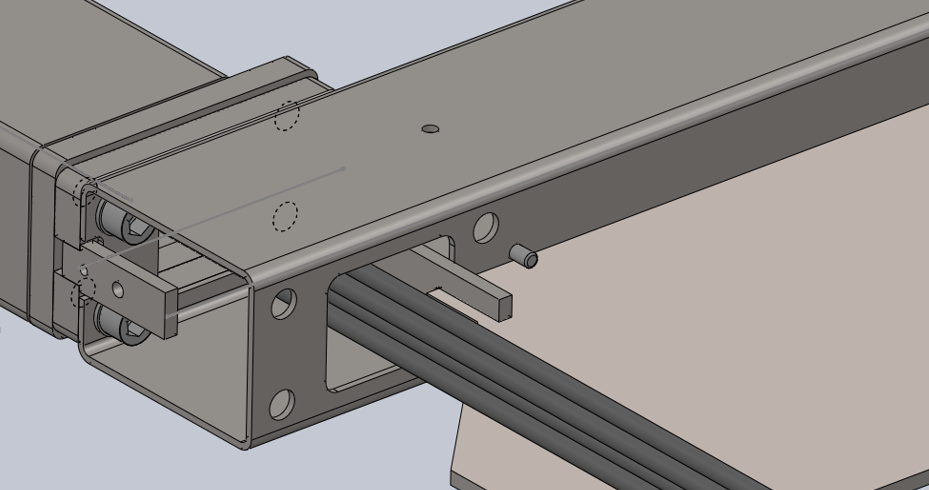
\includegraphics[width=0.50\linewidth]{PD_cable_intube.PNG}
\end{cdrfigure}


%%%%%%%%%%%%%%%%%%%%%%%%%%
\subsection{Alternative photo detector under development}

%\fixme{add citation to bib:
% arapuca_jinst 
%A.A. Machado and E. Segreto, \emph{ARAPUCA a new device for liquid argon scintillation light detection}, {JINST}  {\bf 11} (2016) C02004.
%}
%\section{The ARAPUCA device}
While a sufficient number of the two standard arrays are being produced to fully outfit ProtoDUNE-SP, it is possible that some will bays will have experimental detectors installed in place 
of the 4 standard arrays. One type of detector that is being developed in an attempt to increase the light detection eficiency is called an ARAPUCA.

The ARAPUCA is a device based on a new technology that should allow to collect photons with a window of big area with detection efficiencies at the level of several percent while using 
active photon detectors with much smaller area.
The fundamental idea at the basis of the ARAPUCA is to trap photons inside a box with highly reflective internal surfaces, so that the detection efficiency of trapped photons is high even with a  limited active coverage of its internal surface \cite{arapuca_jinst}.

Photons trapping is achieved by using a clever wavelength-shifting technique coupled with the technology of the dichroic shortpass optical filters. The latter are multilayer acrylic films 
with the  property of being highly transparent to photons with a wavelength below a tunable cut-off while being almost perfectly reflective to photons with wavelength above the cut-off. 
A dichroic shortpass filter deposited with two different wavelength shifters (one on each side) will be the core of the device. In particular, it will be the acceptance window of the 
ARAPUCA. The rest of the device will be a flattened box with highly reflective internal surfaces (PTFE, 3M-VIKUITI ESR, \dots), closed on the top by the 
dichroic  filter deposited with the two shifters. A fraction of the box internal surface is occupied by the active photo-sensors (Silicon Photomultipliers - SiPM) which will detect the trapped photons.

Two arrays of small ARAPUCAs will be installed in the detector %inside protoDUNE 
to test the devices in a real experimental situation and to directly compare their performances with those of the guiding 
bars and other eventual alternative photon detection schemes.\
The arrays will be compatible with the mechanical solutions foreseen for the guiding bars and will have zero impact on the construction of the detector. In particular each one of the two 
arrays will replace one bar. It will be composed by eight ARAPUCAs/bar (for a total of 16 devices)  as shown in Figure~\ref{fig:arapuca_array}.
%*****************************FIGURE 2*****************************%
\begin{cdrfigure}[ARAPUCA array installed in a APA frame]
  {arapuca_array}{One ARAPUCA array of eight devices installed in a APA frame in place of a scintillating bar.}
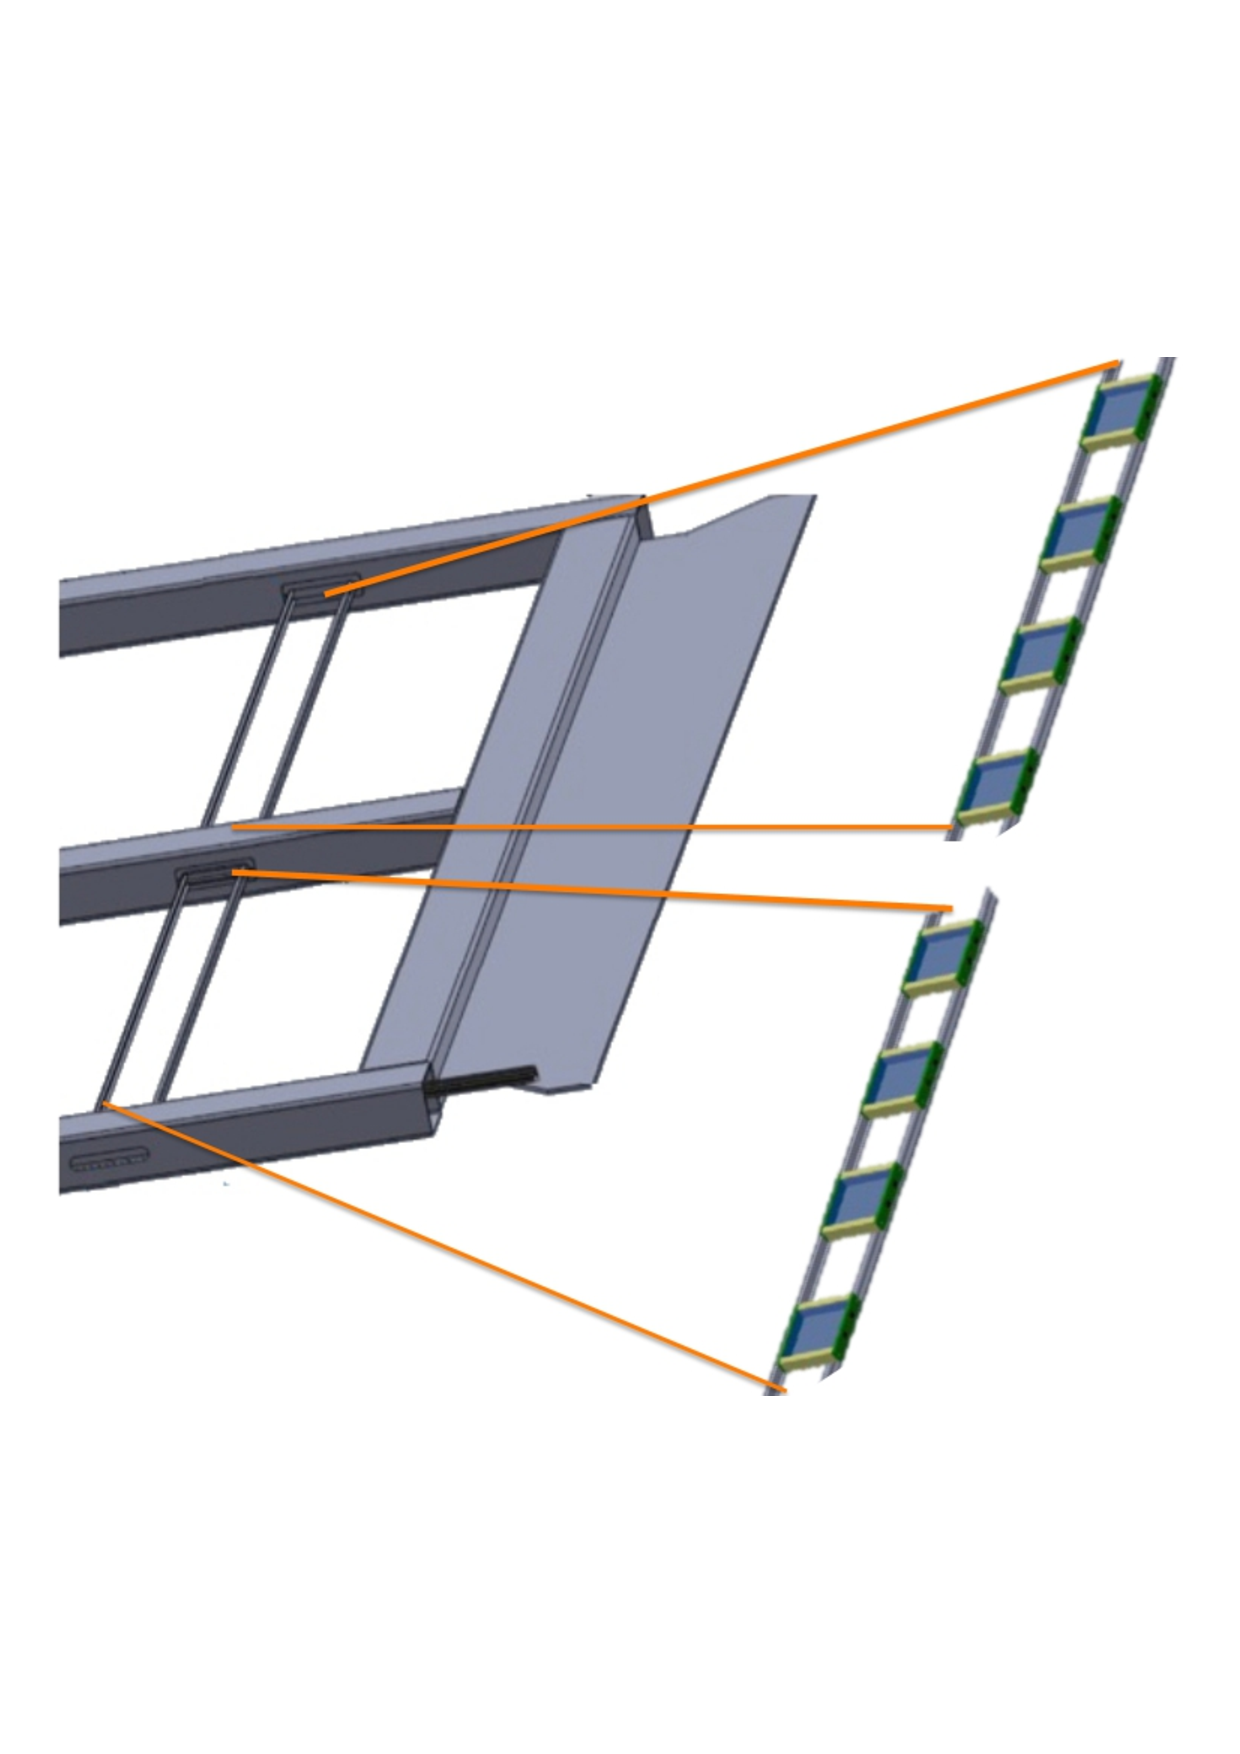
\includegraphics[width=0.50\linewidth]{APA_ARAPUCA}
\end{cdrfigure}

%***********************************************************************%
Each ARAPUCA will be a teflon box with dimensions of 5$\times$5$\times$1 cm$^3$ with an acceptance window of 5$\times$5 
cm$^2$ and the trapped light will be detected by 2 SIPM (SensL 60035 - 6$\times$6 mm$^2$ active area each). The readout scheme foresees the ganging of the SiPMs from two ARAPUCAs (4 sensors) so that each array will require 4 channels, which will use the same cabling and the same SSP read-out of the guiding bars.

%%%%%%%%%%%%%%%%%%%%%%%%%%
\subsection{Photon detector UV-light monitoring system}
\label{sec_pd_calib}

\fixme{Need to reduce to 1-2 pages, (flavio)}
%Items relevant to the PDS calibration are the fast and slow components of the light, photon propagation including scattering and reflections, impact of N$_2$, E-field strength, 
%and the energy range of interest. A calibration system that addresses these issues has to be both comprehensive and cost-effective, and has to be tied to the overall 
%calibration system for ProtoDUNE-SP, which includes both charge and scintillation light calibration techniques. 
%In addition, there is a need to evaluate relative efficiencies of multiple PD units and monitor response and stability of the system as a function of time.

A UV-light-based monitoring system that will serve to monitor the relative performance and time resolution of the system has been designed. % and is described here.
The system will consist of a set of UV LEDs as light sources in the VUV wavelength range, coupled to quartz fibers, to transmit light from outside the detector volume to desired locations at the CPA within the TPC.
Light diffusers located at the CPA surface will uniformly illuminate the APA area with photon-detector system (PDS) elements.
The light sources located and fired externally, with fibers running into the cryostat to diffusers that will emit light from the CPA to the APA. 
For the detector %ProtoDUNE-SP cryostat 
at the surface at CERN, the UV light system will be complementary to cosmic ray muon 
tracks and Michel electrons as means of calibration. In terms of light sources the measurements will be performed with an UV (245-280) light source.
The UV light essentially mimics physics, although at a different wavelength starting from the wavelength-shifter conversion, 
light guide propagation, photo-sensor detection and the front-end electronics readout.
	
The external UV-light monitoring system is designed with the following goals:
				
\begin{itemize}
\item Simple to implement (no active components within PD/APA, such as LEDs or fibers mounted within APA).
\item Uniformly illuminates APA surface with the light diffused from CPA locations.
\item Has a potential to be adapted for deployment in a large Far Detector in the future
\end{itemize}

In terms of technical requirements the system needs to:
\begin{itemize}
\item provide light levels down to a single p.e. at individual photon-detector channels,
\item provide higher light levels to test linearity of the PDS,
\item provide variable pulse width to test the time resolution of the photon detector response, and
\item uniformly illuminate the APA area of the detector for relative monitoring of the PDS channels
\end{itemize}

Figure~\ref{fig:fig-c-1} illustrates the system design schematically. The system consists of a 1U rack mount Light Calibration Module (LCM) sitting outside the cryostat. The LCM generates light pulses that propagate through a quartz fiber-optic cable to diffusers at the CPA to distribute the light uniformly across the photon detectors mounted within the APA.  ProtoDUNE-SP will have five light 
diffusers on the CPA plane: one in the center and four diffusers close to the CPA corners. 
%
 \begin{cdrfigure}[UV-light monitoring system]{fig-c-1}{Concept of the UV-light monitoring system for the photon detector in liquid argon.}
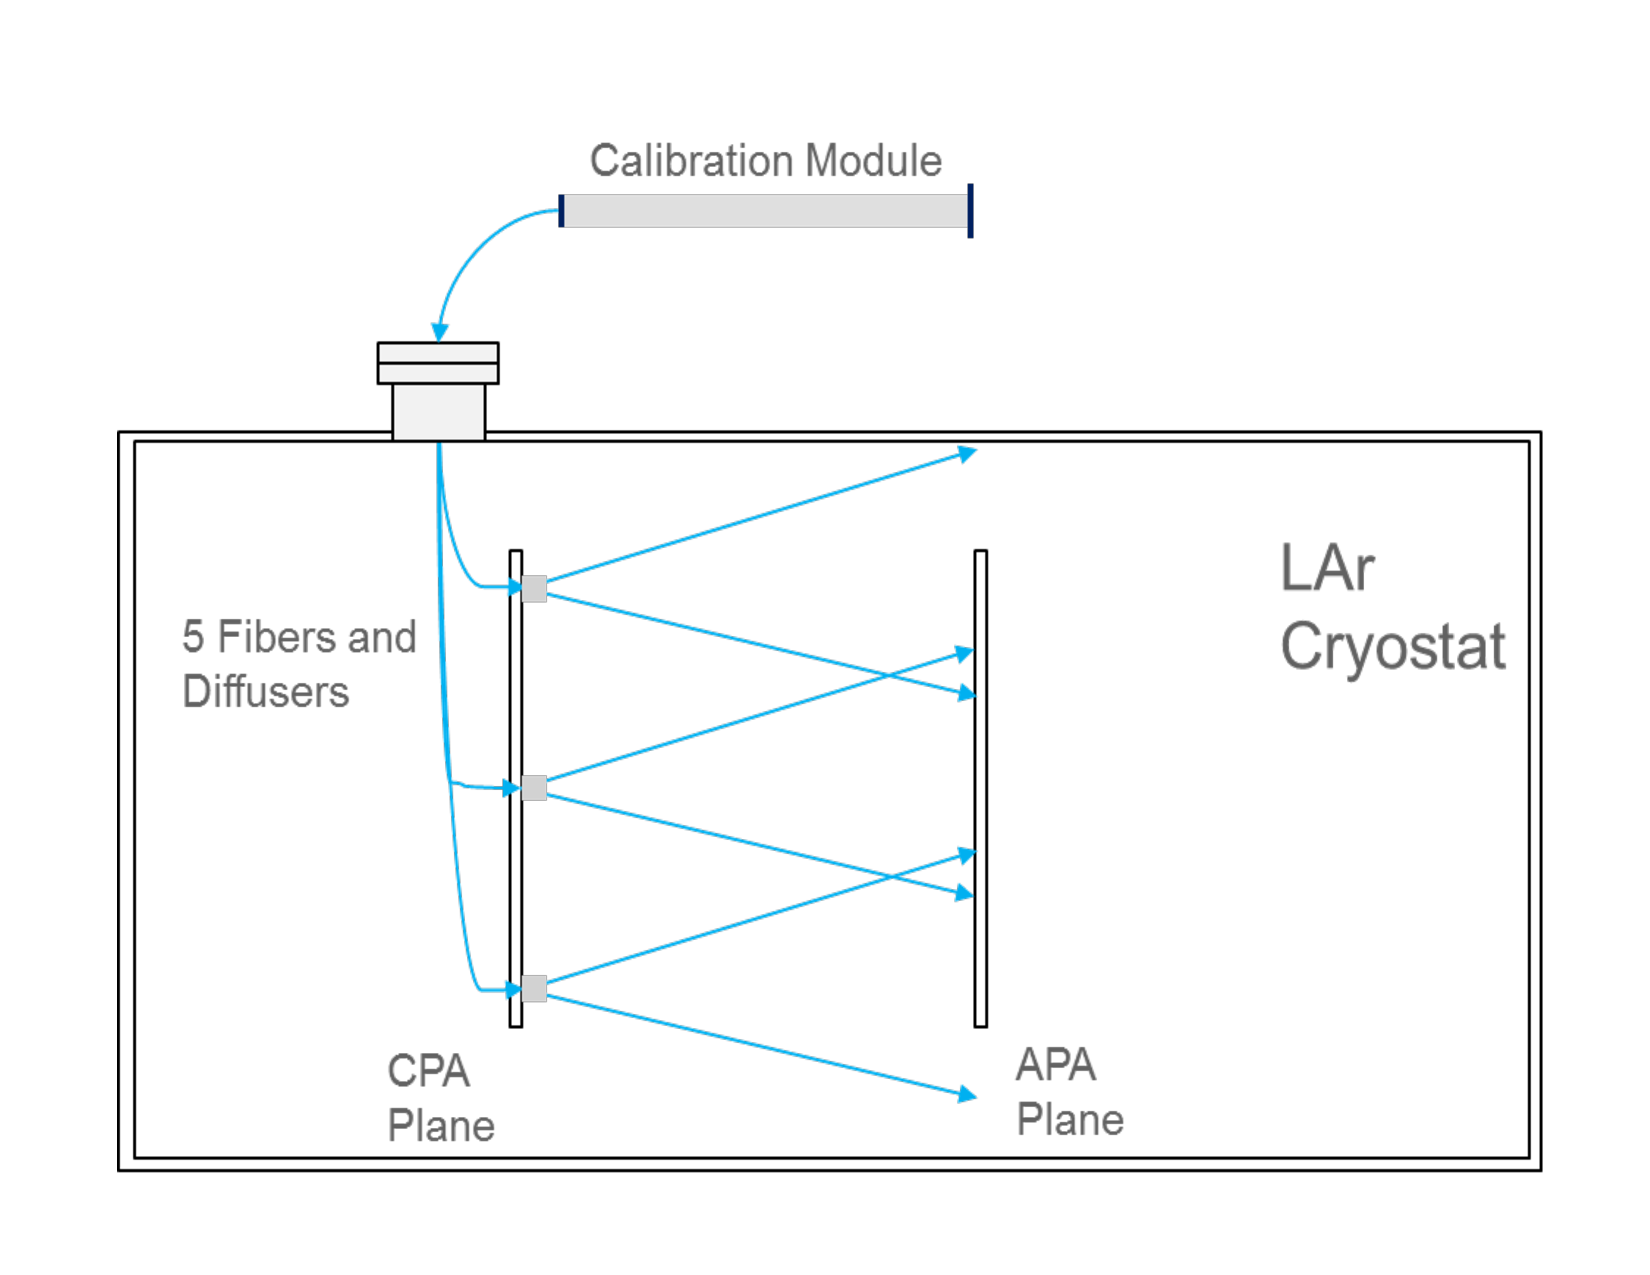
\includegraphics[angle=0,width=0.7\textwidth]{calPD_concept-from-35ton.pdf}
\end{cdrfigure}
%


The LCM utilizes the logic and timing control of the photon-detector readout electronics ("SSP") unit.  
An SSP board was repackaged into a deeper rack mount chassis that accommodates a new internal 
LED Pulser Module (LPM) and an additional bulk power supply. The LPM utilizes five digital outputs from the SSP board to control the LPM pulse and its duration.  
These outputs are derived from the charge injection control logic within the SSP's FPGA.  
The even-channel SiPM bias Digital to Analog Converters (DACs)
are used to control the LPM pulse amplitude.  
The adjacent odd channels are used to read out a reference photodiode used for pulse-by-pulse monitoring of the LED light output.  
The output of the monitoring diode may be used to normalize 
the response of the SiPMs in the detector to the monitoring pulse.


\fixme{A bunch of content removed from here; but then gap in (paper) pages received from Flavio (missing 4-147 to 4-180); not sure what to do with remainder of this file. Anne}

\fixme{How long do these monitoring run take ? When would they be taken (relative to beam and comics running) ? Some interference with light from comics is expected; how will this be addressed ? Time of a flash will be known much better then 1us, so not much overlap with random cosmic events at ~1ms }

The controlled source of light %described here 
in this monitoring system will be used to perform time offset and time resolution measurements.  
Many effects contribute to a finite time resolution, relative time offset of photon-detector channels, scintillation time constants, 
photon conversion with wavelength shifter, photon propagation through photon-detector paddle, SiPM jitter, and FEE resolution. 
Most of these effects are constant and can be individually 
measured on the bench.  The UV light monitoring system will monitor overall stability of the photon detector in both time
and amplitude.
